\subsection{Singleton}


\textbf{Scopo}: Creazionale \\
\textbf{Raggio d'azione}: Oggetti

\paragraph{Definizione} Il pattern Singleton assicura che un classe abbia una sola istanza e fornisca un solo punto di accesso globale a tale istanza.

\paragraph{Problema} In un sistema potrebbero esistere più stampanti, ma potrebbe essere presente soltanto una coda di stampa. In un sistema operativo dovrebbe essere presente solo un file system e un solo window manager

\paragraph{Soluzione} Per assicurare che una classe abbia una sola istanza e che tale istanza sia facilmente accessibile per gli utilizzatori si può fare in modo che la classe stessa abbia la responsabilità di creare le proprie istanze. La classe può assicurare che nessun’altra istanza possa essere creata e può fornire un modo semplice per accedere all’istanza.

\begin{figure}[H]
    \centering
    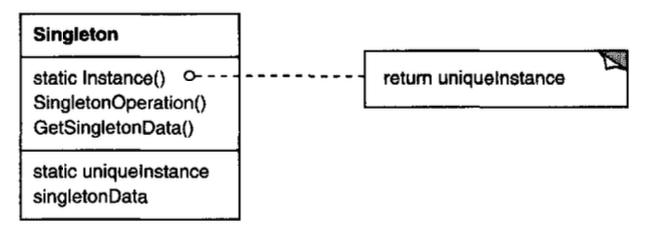
\includegraphics[width=0.4\linewidth]{assets/pattern/singleton/singleton-struttura.png}
\end{figure}

\paragraph{Struttura e Conseguenze} Il pattern risulta essere applicabile in due casi in particolare:
\begin{itemize}
    \item Quando deve esistere esattamente un’istanza di una classe resa accessibile ai client attraverso un punto di accesso noto a tutti gli utilizzatori.
    \item Quando l’unica istanza deve poter essere estesa attraverso la definizione di sottoclassi ed i client devono essere in grado di utilizzare le istanze estese senza dover modificare il proprio codice.
\end{itemize}

\textbf{Java}

\begin{minted}[
    fontsize=\footnotesize,
    linenos,
]{java}
public final class Singleton { 
    private static Singleton INSTANCE = null; 
    
    private Singleton(){} 
    
    public static synchronized Singleton getInstance() { 
        if (INSTANCE == null) { 
            INSTANCE=new Singleton(); 
        } 
        return INSTANCE; 
    } 
}
\end{minted}

\newpage